\documentclass[tikz]{standalone}

\usepackage{amsmath, amssymb, MnSymbol}
\usepackage{tikz}
\usetikzlibrary{shapes.geometric, arrows, calc, positioning}

\tikzset{XOR/.style={draw,circle,append after command={
        [shorten >=\pgflinewidth, shorten <=\pgflinewidth,]
        (\tikzlastnode.north) edge (\tikzlastnode.south)
        (\tikzlastnode.east) edge (\tikzlastnode.west)
        }
    }
}

\tikzset{BXOR/.style={draw,rectangle,append after command={
        [shorten >=\pgflinewidth, shorten <=\pgflinewidth,]
        (\tikzlastnode.north) edge (\tikzlastnode.south)
        (\tikzlastnode.east) edge (\tikzlastnode.west)
        }
    }
}

\newcommand{\SBOX}{\text{SBOX}}
\newcommand{\rot}{\text{rot11}}

\tikzstyle{block} = [draw, fill=white, rectangle,
    minimum width=1cm, minimum height=0.5cm]

\begin{document}
    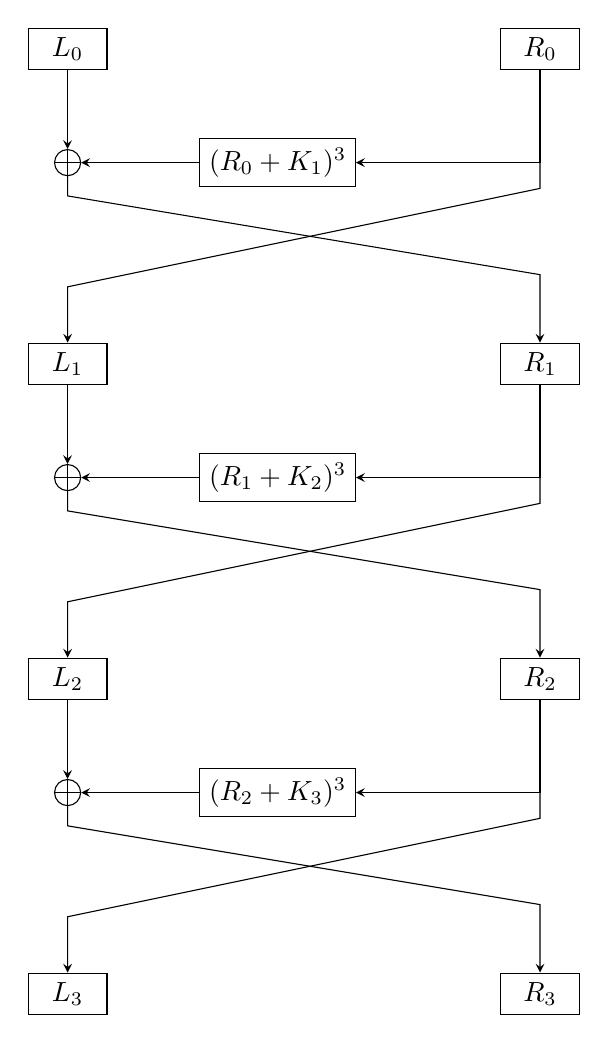
\begin{tikzpicture}[node distance=2cm]
        %Round 1
        \node [block] (L0) at (0, 0) {$L_0$};
        \node [block] (R0) at (6, 0) {$R_0$};
        \node [XOR, below=1cm of L0] (x0) {};
        \node [block, right=1.5cm of x0] (F0) {$(R_0 + K_1)^3$};

        %Round 2
        \node [block] (L1) at (0, -4) {$L_1$};
        \node [block] (R1) at (6, -4) {$R_1$};
        \node [XOR, below=1cm of L1] (x1) {};
        \node [block, right=1.5cm of x1] (F1) {$(R_1 + K_2)^3$};
        
        %Round 3
        \node [block] (L2) at (0, -8) {$L_2$};
        \node [block] (R2) at (6, -8) {$R_2$};
        \node [XOR, below=1cm of L2] (x2) {};
        \node [block, right=1.5cm of x2] (F2) {$(R_2 + K_3)^3$};

        %Round 4
        \node [block] (L3) at (0, -12) {$L_3$};
        \node [block] (R3) at (6, -12) {$R_3$};

        \draw [-stealth] (L0) -- (x0);
        \draw [stealth-] (x0) -- (F0);
        \draw [-stealth] (R0) |- (F0);
        \draw [-stealth] (R0.south) -- ++(0, -1.5) 
                -- ++(-6, -1.25) -| (L1.north);
        \draw [-stealth] (x0.south) -- ++(0, -0.25)
                -- ++(6, -1) -| (R1.north);

        \draw [-stealth] (L1) -- (x1);
        \draw [stealth-] (x1) -- (F1);
        \draw [-stealth] (R1) |- (F1);
        \draw [-stealth] (R1.south) -- ++(0, -1.5) 
                -- ++(-6, -1.25) -| (L2.north);
        \draw [-stealth] (x1.south) -- ++(0, -0.25)
                -- ++(6, -1) -| (R2.north);
        
        \draw [-stealth] (L2) -- (x2);
        \draw [stealth-] (x2) -- (F2);
        \draw [-stealth] (R2) |- (F2);
        \draw [-stealth] (R2.south) -- ++(0, -1.5) 
                -- ++(-6, -1.25) -| (L3.north);
        \draw [-stealth] (x2.south) -- ++(0, -0.25)
                -- ++(6, -1) -| (R3.north);
    %     \draw [-stealth] (L1) -- (x1);
    %     \draw [stealth-] (x1) -- (s1);
    %     \draw [stealth-] (s1) -- (sb1);
    %     \draw [stealth-] (sb1) -- (b1);
    %     \draw [-stealth] (K1) -- (b1);
    %     \draw [-stealth] (R1) |- (b1);
        
    %     \draw [-stealth] (Li) -- (xi);
    %     \draw [stealth-] (xi) -- (si);
    %     \draw [stealth-] (si) -- (sbi);
    %     \draw [stealth-] (sbi) -- (bi);
    %     \draw [-stealth] (Ki) -- (bi);
    %     \draw [-stealth] (Ri) |- (bi);
    %     \draw [-stealth] (Lt.south) -- ++(0, -0.25)
    %             -- ++(5.25, -1) -| (Ri.north);
    %     \draw [-stealth] (Rt.south) -- ++(0, -0.25)
    %            -- ++(-5.25, -1) -| (Li.north);

    %     \draw [-stealth] (xi.south) -- ++(0, -0.25)
    %            -- ++(5.25, -1) -| (R.north);
    %    \draw [-stealth] (Ri.south) -- ++(0, -1.5)
    %           -- ++(-5.25, -1) -| (L.north);
    \end{tikzpicture}
\end{document}